% ============================================================
% 10. SYSTEM ARCHITECTURE
% ============================================================

\begin{sectionintro}{10}{System Architecture}{
  \begin{itemize}[leftmargin=1.5em]
    \item High-level three-tier architecture overview
    \item Component interactions and data flow
    \item Security boundaries and trust zones
    \item Scalability and deployment architecture
    \item Integration patterns and interfaces
  \end{itemize}
}
\lettrine[lines=3, lhang=0.1, loversize=0.15]{\color{primaryBlue}A}{rchitecture defines how system components collaborate} to achieve functional and non-functional requirements. This chapter presents zGate's layered architecture, examining the gateway server, CLI client, and web dashboard in detail. The design emphasizes clear separation of concerns, security by design, and maintainability while implementing Zero Trust principles throughout.
\end{sectionintro}

\chapter{System Architecture}

This chapter provides a comprehensive technical overview of the zGate platform architecture, detailing the design and implementation of each component. The system follows a layered architecture pattern with clear separation of concerns, implementing Zero Trust principles at the database protocol level.

% ============================================================
\section{High-Level Architecture}
% This section is reserved for high-level architecture diagram and overview
% To be completed by teammate

% ============================================================
\section{Detailed Architecture}

The zGate platform is architected as a distributed system comprising three primary components: the Gateway Server, Web UI, and CLI. Each component is designed with specific responsibilities that collectively implement Zero Trust database access.

\subsection{System Components Overview}

The zGate architecture can be conceptualized as a multi-layered security gateway that intercepts, validates, and controls all database access. Figure~\ref{fig:complete-system-flow} illustrates the complete data flow across all system components.

\begin{figure}[H]
    \centering
    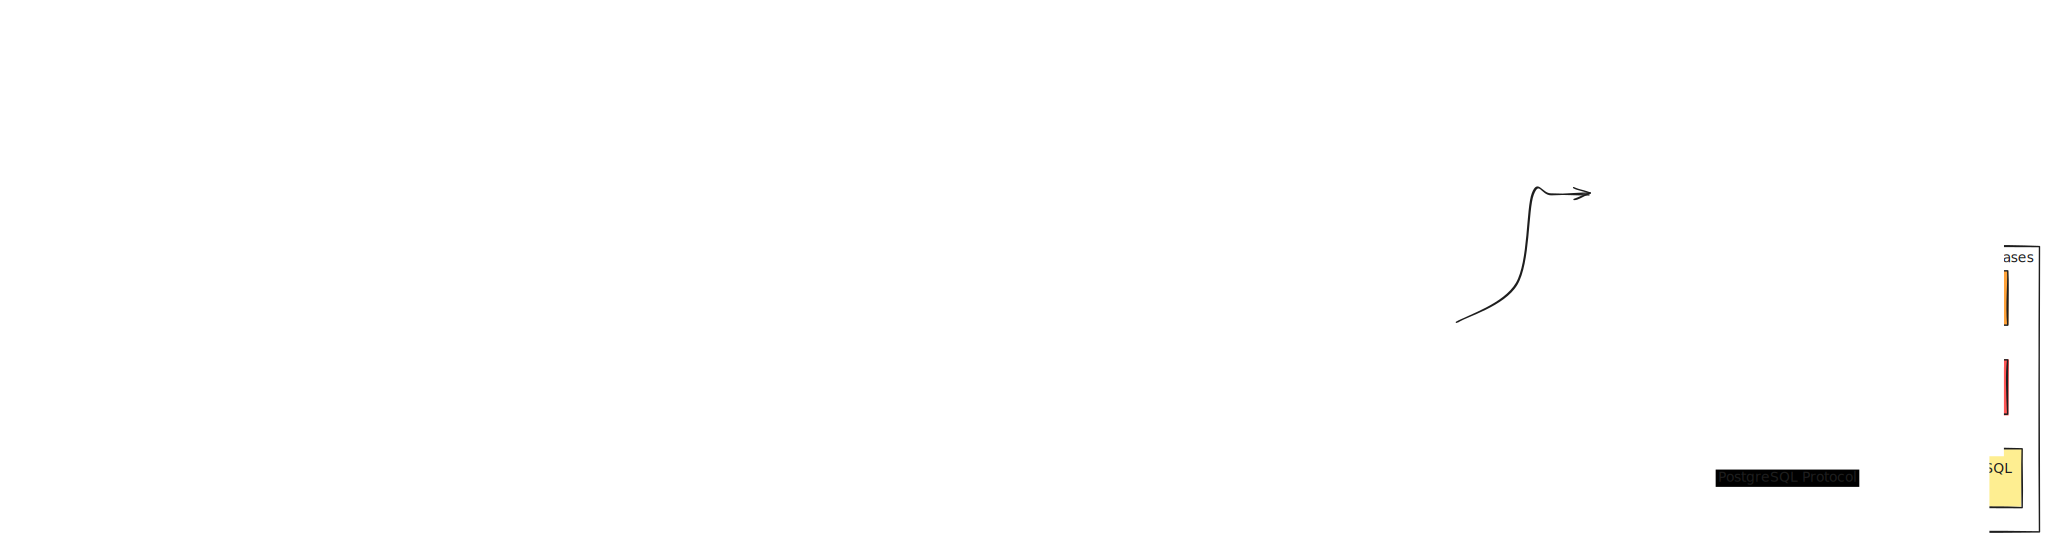
\includegraphics[width=0.95\textwidth]{images/images for doc/Complete system data flow.png}
    \caption{Complete System Data Flow Architecture}
    \label{fig:complete-system-flow}
\end{figure}

The system architecture follows a clear separation of concerns:

\begin{itemize}[leftmargin=*]
    \item \textbf{Client Layer:} WebUI and CLI provide user interfaces for authentication and database connection management
    \item \textbf{API Layer:} RESTful API server handles authentication, authorization, and session management
    \item \textbf{Gateway Layer:} Protocol-aware proxy intercepts and controls database traffic
    \item \textbf{Data Layer:} Target databases are accessed through the gateway with enforced security policies
    \item \textbf{Storage Layer:} SQLite database stores users, roles, permissions, and audit logs
\end{itemize}

% ============================================================
\subsection{Gateway and Proxy Components}

The Gateway Server is the heart of the zGate platform, implementing wire-protocol level database proxying with comprehensive security controls. It is architected as a collection of specialized components, each with distinct responsibilities.

\subsubsection{Component Architecture}

The gateway implements a modular pipeline architecture with the following core components:

\begin{figure}[H]
\centering
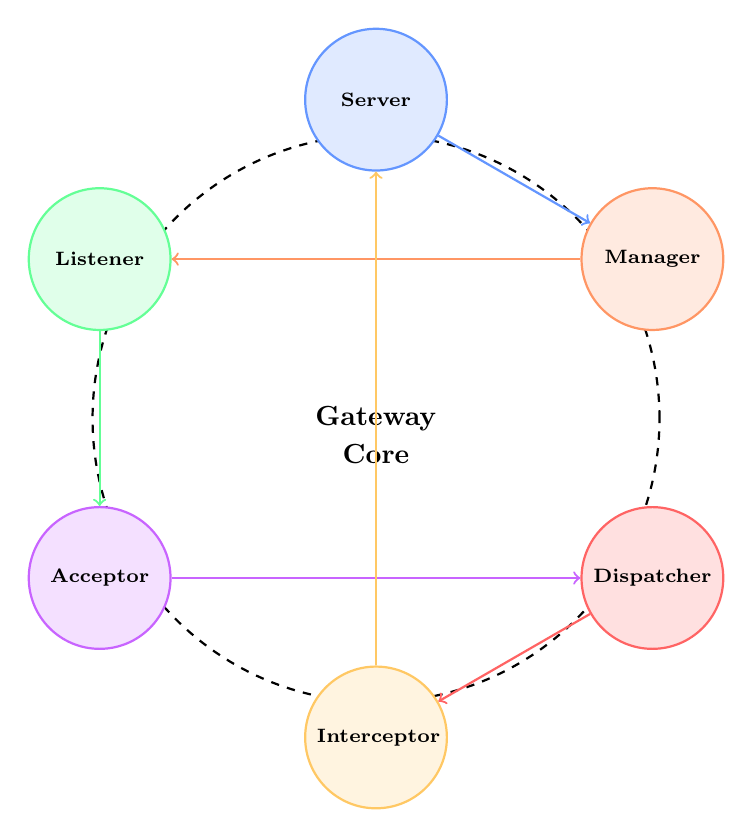
\begin{tikzpicture}[scale=0.9]
    % Define colors
    \definecolor{servercolor}{RGB}{100, 150, 255}
    \definecolor{managercolor}{RGB}{255, 150, 100}
    \definecolor{listenercolor}{RGB}{100, 255, 150}
    \definecolor{acceptorcolor}{RGB}{200, 100, 255}
    \definecolor{dispatchercolor}{RGB}{255, 100, 100}
    \definecolor{interceptorcolor}{RGB}{255, 200, 100}
    
    % Central circle
    \draw[thick, dashed] (0,0) circle (4cm);
    \node at (0, 0) {\textbf{Gateway}};
    \node at (0, -0.5) {\textbf{Core}};
    
    % Component circles arranged in a circle
    % Server (top)
    \node[circle, draw=servercolor, fill=servercolor!20, thick, minimum size=1.8cm, align=center, text width=1.5cm] (server) at (0, 4.5) {\textbf{\scriptsize Server}};
    
    % Manager (top-right)
    \node[circle, draw=managercolor, fill=managercolor!20, thick, minimum size=1.8cm, align=center, text width=1.5cm] (manager) at (3.9, 2.25) {\textbf{\scriptsize Manager}};
    
    % Dispatcher (bottom-right)
    \node[circle, draw=dispatchercolor, fill=dispatchercolor!20, thick, minimum size=1.8cm, align=center, text width=1.5cm] (dispatcher) at (3.9, -2.25) {\textbf{\scriptsize Dispatcher}};
    
    % Interceptor (bottom)
    \node[circle, draw=interceptorcolor, fill=interceptorcolor!20, thick, minimum size=1.8cm, align=center, text width=1.5cm] (interceptor) at (0, -4.5) {\textbf{\scriptsize Interceptor}};
    
    % Acceptor (bottom-left)
    \node[circle, draw=acceptorcolor, fill=acceptorcolor!20, thick, minimum size=1.8cm, align=center, text width=1.5cm] (acceptor) at (-3.9, -2.25) {\textbf{\scriptsize Acceptor}};
    
    % Listener (top-left)
    \node[circle, draw=listenercolor, fill=listenercolor!20, thick, minimum size=1.8cm, align=center, text width=1.5cm] (listener) at (-3.9, 2.25) {\textbf{\scriptsize Listener}};
    
    % Arrows showing data flow
    \draw[->, thick, servercolor] (server) -- (manager);
    \draw[->, thick, managercolor] (manager) -- (listener);
    \draw[->, thick, listenercolor] (listener) -- (acceptor);
    \draw[->, thick, acceptorcolor] (acceptor) -- (dispatcher);
    \draw[->, thick, dispatchercolor] (dispatcher) -- (interceptor);
    \draw[->, thick, interceptorcolor] (interceptor) -- (server);
\end{tikzpicture}
\caption{Gateway Component Architecture and Data Flow}
\label{fig:gateway-components}
\end{figure}

\begin{enumerate}[leftmargin=*]
    \item \textbf{Server:} Orchestrates the lifecycle of database handlers and manages protocol-specific processing
    \item \textbf{Listener:} Manages TCP listener lifecycle for dynamic port allocation per user session
    \item \textbf{Acceptor:} Handles incoming client connections and establishes connection metadata
    \item \textbf{Dispatcher:} Establishes backend database connections and manages bidirectional traffic forwarding
    \item \textbf{Manager:} Coordinates session lifecycle, credential provisioning, and resource cleanup
    \item \textbf{Interceptor Chain:} Provides composable query processing pipeline for security enforcement
\end{enumerate}

\paragraph{Server Component}

The Server component (\texttt{internal/gateway/server.go}) serves as the orchestration layer for the gateway. Its primary responsibilities include:

\begin{itemize}[leftmargin=*]
    \item \textbf{Handler Initialization:} Pre-initializes protocol handlers for all registered database types (MySQL, PostgreSQL, MSSQL, MariaDB)
    \item \textbf{TLS Configuration:} Manages end-to-end TLS encryption for proxy-to-database connections with support for certificate pinning
    \item \textbf{Handler Registry:} Maintains a type-to-handler mapping that enables protocol-specific processing
    \item \textbf{Resource Sharing:} Provides thread-safe access to shared handlers across multiple sessions
\end{itemize}

\textbf{Input:} Database configurations from SQLite store, TLS certificate paths\\
\textbf{Output:} Initialized handlers for each database type\\
\textbf{Communication:} Provides handlers to Manager component via GetHandler() method

\paragraph{Manager Component}

The Manager component (\texttt{internal/proxy/manager.go}) implements the session lifecycle management with sophisticated credential provisioning logic. It follows a three-tier account priority system:

\begin{enumerate}[leftmargin=*]
    \item \textbf{Personal Accounts:} Dedicated database accounts assigned to specific users
    \item \textbf{Shared Accounts:} Pool of pre-created accounts shared across users with concurrent usage limits
    \item \textbf{Ephemeral Accounts:} Temporary accounts created on-demand and destroyed on disconnect
\end{enumerate}

\textbf{Session Creation Workflow:}
\begin{enumerate}[leftmargin=*]
    \item Validates user permissions for requested database using real-time policy evaluation
    \item Attempts to retrieve personal database account from store
    \item If unavailable, checks shared account pool for available credentials
    \item If pool exhausted, creates ephemeral temporary database user with scoped permissions
    \item Allocates dynamic port from operating system
    \item Initializes session context and starts listener
    \item Returns connection details to API layer
\end{enumerate}

\textbf{Input:} JWT claims, database name, user permissions\\
\textbf{Output:} Session object with port, credentials, account type\\
\textbf{Communication:} Interacts with Store for credentials, Gateway Server for handlers, Database for ephemeral user creation

\paragraph{Listener Component}

The Listener component (\texttt{internal/gateway/listener.go}) manages the TCP listener lifecycle for each user session. Each session receives a dedicated listener on a dynamically allocated port.

\textbf{Key Responsibilities:}
\begin{itemize}[leftmargin=*]
    \item Creates TCP listener on specified port (0.0.0.0:port for remote mode, configurable for security)
    \item Accepts incoming client connections in a loop
    \item Delegates each connection to Acceptor for processing
    \item Implements graceful shutdown via context cancellation
    \item Tracks active connections using WaitGroup for clean termination
\end{itemize}

\textbf{Input:} Listen address, database configuration, session metadata\\
\textbf{Output:} Accepted client connections\\
\textbf{Communication:} Spawns Acceptor for each connection

\paragraph{Acceptor Component}

The Acceptor component (\texttt{internal/gateway/acceptor.go}) processes each incoming client connection from acceptance to completion.

\textbf{Responsibilities:}
\begin{itemize}[leftmargin=*]
    \item Captures client connection metadata (IP address, timestamp)
    \item Associates connection with session ID for audit correlation
    \item Creates ConnectionMetadata structure with user context
    \item Delegates to Dispatcher for protocol handshake and traffic forwarding
    \item Ensures proper connection cleanup on termination
\end{itemize}

\textbf{Input:} Client TCP connection, database credentials, session metadata\\
\textbf{Output:} ConnectionMetadata structure\\
\textbf{Communication:} Instantiates Dispatcher for bidirectional proxying

\paragraph{Dispatcher Component}

The Dispatcher component (\texttt{internal/gateway/dispatcher.go}) is responsible for establishing backend connections and managing the entire query lifecycle.

\textbf{Connection Establishment:}
\begin{enumerate}[leftmargin=*]
    \item Establishes TCP connection to backend database server
    \item Configures protocol handler with target database and proxy credentials
    \item Performs authentication handshake using real database credentials
    \item Handles TLS upgrade for both client-proxy and proxy-backend connections
    \item Extracts upgraded connections from handshake result
\end{enumerate}

\textbf{Query Processing Loop:}
\begin{enumerate}[leftmargin=*]
    \item Reads command from client connection using protocol handler
    \item Creates QueryContext with session metadata
    \item Invokes BeforeQuery interceptor chain (safety checks, logging)
    \item Forwards allowed queries to backend database
    \item Receives query results from database
    \item Invokes AfterQuery interceptor chain (masking, logging)
    \item Forwards processed results back to client
\end{enumerate}

\textbf{Input:} Client and backend connections, database credentials, interceptor configuration\\
\textbf{Output:} Processed query results with security enforcement applied\\
\textbf{Communication:} Coordinates between Protocol Handler, Interceptor Chain, and both client and database

\paragraph{Interceptor Chain}

The Interceptor Chain (\texttt{internal/proxy/interceptor/}) implements a composable pipeline for query processing with three primary interceptors:

\begin{tcolorbox}[colback=blue!5!white, colframe=blue!75!black, title=\textbf{1. Logging Interceptor}]
\textbf{Purpose:} Provides comprehensive audit trail for all database operations

\textbf{Functionality:}
\begin{itemize}[leftmargin=*]
    \item Captures query text, timestamp, user identity, target database
    \item Records query execution duration and rows affected
    \item Filters internal/system queries (SET, SHOW, SELECT @@)
    \item Writes structured logs to file for compliance and forensics
\end{itemize}

\textbf{Input:} QueryContext before execution\\
\textbf{Output:} Structured log entry
\end{tcolorbox}

\begin{tcolorbox}[colback=red!5!white, colframe=red!75!black, title=\textbf{2. Safety Interceptor}]
\textbf{Purpose:} Prevents dangerous database operations based on configurable rules

\textbf{Blocked Operations:}
\begin{itemize}[leftmargin=*]
    \item DELETE without WHERE clause (mass deletion)
    \item UPDATE without WHERE clause (mass update)
    \item TRUNCATE TABLE (complete data loss)
    \item DROP TABLE/DATABASE (schema destruction)
    \item ALTER TABLE (schema modification)
    \item CREATE statements (schema creation)
    \item GRANT/REVOKE (privilege escalation)
\end{itemize}

\textbf{Input:} Query text from QueryContext\\
\textbf{Output:} BLOCK decision or ALLOW with logged warning
\end{tcolorbox}

\begin{tcolorbox}[colback=green!5!white, colframe=green!75!black, title=\textbf{3. Masking Interceptor}]
\textbf{Purpose:} Dynamically masks sensitive data in query results based on column names

\textbf{Masking Rules:}
\begin{itemize}[leftmargin=*]
    \item \textbf{Email:} First character + domain visible (e.g., j***@email.com)
    \item \textbf{Phone/Mobile:} Last 4 digits visible (e.g., *****1234)
    \item \textbf{Credit Card/SSN:} Last 4 digits visible
    \item \textbf{Password/Secret/Token:} Full redaction (*****)
    \item \textbf{Name fields:} First letter only (e.g., J****)
\end{itemize}

\textbf{Input:} Query result set with column metadata\\
\textbf{Output:} Masked result set with sensitive values redacted
\end{tcolorbox}

\textbf{Composite Interceptor:} The CompositeInterceptor orchestrates the execution of all configured interceptors in sequence, maintaining the chain of responsibility pattern.

% ============================================================
\subsection{Configuration Flow}

Figure~\ref{fig:config-flow} illustrates the system initialization and configuration flow that occurs when the zGate Gateway Server starts.

\begin{figure}[H]
    \centering
    \includegraphics[width=0.35\textwidth]{images/images for doc/System Configuration.png}
    \caption{System Configuration and Initialization Flow}
    \label{fig:config-flow}
\end{figure}

The configuration process ensures all components are properly initialized before accepting client connections:

\begin{enumerate}[leftmargin=*]
    \item \textbf{Store Initialization:} SQLite database is opened and schema migrations are applied
    \item \textbf{Gateway Server Creation:} All database type handlers are pre-initialized
    \item \textbf{TLS Configuration:} Certificates are loaded for end-to-end encryption
    \item \textbf{API Server Initialization:} RESTful endpoints are registered with middleware
    \item \textbf{Manager Creation:} Session management component is instantiated with store and gateway references
    \item \textbf{Logger Setup:} Structured logging is configured with appropriate verbosity levels
    \item \textbf{Server Listening:} API server starts accepting HTTP requests
\end{enumerate}

% ============================================================
\subsection{Authentication System}

The authentication system implements JWT-based token authentication with automatic token rotation for enhanced security. The system supports both user and admin authentication flows.

\subsubsection{User Login Flow}

Figure~\ref{fig:user-login} depicts the user authentication process used by both CLI and WebUI components.

\begin{figure}[H]
    \centering
    \includegraphics[width=0.85\textwidth]{images/images for doc/Authentication flows/2.1 User Login Flow (CLI & WebUI).png}
    \caption{User Authentication Flow}
    \label{fig:user-login}
\end{figure}

\textbf{Authentication Process:}
\begin{enumerate}[leftmargin=*]
    \item Client submits credentials to POST /api/login endpoint
    \item API invokes Authenticator component to verify password using bcrypt
    \item Store retrieves user data and associated role permissions
    \item Authenticator combines role-based and custom permissions
    \item JWT Generator creates short-lived access token (15 minutes expiration)
    \item Store creates refresh token (7 day expiration) linked to user session
    \item Response includes both tokens, token type, expiration, and username
    \item Client stores tokens securely (OS keyring for CLI, memory for WebUI)
\end{enumerate}

\subsubsection{Token Refresh Flow}

Figure~\ref{fig:token-refresh} shows the token refresh mechanism that implements automatic token rotation for security.

\begin{figure}[H]
    \centering
    \includegraphics[width=0.85\textwidth]{images/images for doc/Authentication flows/2.2 Token Refresh Flow.png}
    \caption{Token Refresh Flow with Rotation}
    \label{fig:token-refresh}
\end{figure}

\textbf{Token Rotation Security:}
\begin{itemize}[leftmargin=*]
    \item Client submits current refresh token to POST /api/refresh endpoint
    \item Store validates refresh token and retrieves associated username
    \item New access token is generated with updated permissions
    \item New refresh token is created to replace the old one
    \item Old refresh token is immediately revoked in database
    \item Both new tokens are returned to client
    \item Prevents token reuse attacks and limits blast radius of token compromise
\end{itemize}

\subsubsection{Admin Login Flow}

Figure~\ref{fig:admin-login} illustrates the administrative authentication flow with fallback mechanism.

\begin{figure}[H]
    \centering
    \includegraphics[width=0.85\textwidth]{images/images for doc/Authentication flows/2.3 Admin Login Flow.png}
    \caption{Admin Authentication with User Fallback}
    \label{fig:admin-login}
\end{figure}

\textbf{Dual Authentication Strategy:}
\begin{enumerate}[leftmargin=*]
    \item First attempts admin authentication via dedicated admins table
    \item If admin credentials valid, sets isAdmin flag to true in response
    \item If not found in admins table, falls back to regular user authentication
    \item Returns isAdmin flag indicating permission level for dashboard routing
    \item Updates admin last login timestamp for audit purposes
\end{enumerate}

% ============================================================
\subsection{Database Connection Lifecycle}

The database connection lifecycle implements the core Zero Trust principle: users never handle production credentials. The system manages three types of database accounts with different lifecycle characteristics.

\subsubsection{Database Account Types}

The zGate platform implements a sophisticated three-tier account management system that eliminates credential exposure while optimizing resource utilization and security. Each account type serves a distinct purpose in the Zero Trust architecture:

\paragraph{Personal Database Accounts}

Personal accounts represent the highest privilege tier, providing dedicated database credentials assigned exclusively to individual users.

\textbf{Creation and Provisioning:}
\begin{itemize}[leftmargin=*]
    \item Administrators pre-create accounts through the WebUI administrative interface
    \item Each account is permanently associated with a specific user via user\_id mapping
    \item Credentials are stored encrypted in the zGate database
    \item Account permissions are configured at the database level by DBAs
\end{itemize}

\textbf{Usage Scenario:}
\begin{itemize}[leftmargin=*]
    \item When a user with a personal account requests database access, zGate immediately retrieves their dedicated credentials
    \item No account creation overhead or waiting time
    \item User maintains consistent database identity across sessions
    \item Ideal for privileged users, developers, or users requiring specific database roles
\end{itemize}

\textbf{Lifecycle and Advantages:}
\begin{itemize}[leftmargin=*]
    \item Accounts persist indefinitely across sessions and disconnections
    \item Provides accountability through consistent database audit trails
    \item Enables fine-grained permission management at the user level
    \item Eliminates runtime account provisioning latency
\end{itemize}

\paragraph{Shared Account Pool}

Shared accounts implement a connection pool pattern, enabling multiple users to share a limited set of pre-provisioned database accounts.

\textbf{Creation and Pool Management:}
\begin{itemize}[leftmargin=*]
    \item Administrators create a pool of generic database accounts via WebUI
    \item Each account has configurable concurrent usage limits (max\_concurrent\_users)
    \item Pool size is determined by anticipated concurrent load
    \item Accounts are tagged as \texttt{shared} in the account type field
\end{itemize}

\textbf{Usage Scenario:}
\begin{itemize}[leftmargin=*]
    \item When a user without a personal account connects, zGate queries the pool for available accounts
    \item An account is considered available if \texttt{currently\_in\_use < max\_concurrent\_users}
    \item Upon assignment, the \texttt{currently\_in\_use} counter is atomically incremented
    \item Multiple users can share the same database account simultaneously within the limit
    \item Ideal for read-only users, analysts, or scenarios with many concurrent users
\end{itemize}

\textbf{Lifecycle and Advantages:}
\begin{itemize}[leftmargin=*]
    \item Accounts remain persistent but are released back to the pool on disconnect
    \item The \texttt{currently\_in\_use} counter is decremented when the session ends
    \item Significantly reduces database account sprawl compared to per-user accounts
    \item Optimizes resource utilization in environments with high user counts
    \item Provides a balance between security and operational overhead
\end{itemize}

\paragraph{Ephemeral Temporary Accounts}

Ephemeral accounts represent the ultimate Zero Trust approach: credentials that exist only for the duration of a single database session.

\textbf{Creation and Provisioning:}
\begin{itemize}[leftmargin=*]
    \item Created on-demand by the Gateway Manager component when no personal or shared accounts are available
    \item zGate connects to the database using a privileged provisioning account
    \item Executes \texttt{CREATE USER} with a cryptographically random username and password
    \item Grants appropriate permissions based on the user's role permissions from zGate
    \item Account details are stored only in memory within the active session context
\end{itemize}

\textbf{Usage Scenario:}
\begin{itemize}[leftmargin=*]
    \item Triggered when personal account doesn't exist and shared pool is exhausted
    \item Entire account lifecycle contained within a single zGate session
    \item User never sees or handles the actual database credentials
    \item Ideal for untrusted environments or maximum security requirements
\end{itemize}

\textbf{Lifecycle and Advantages:}
\begin{itemize}[leftmargin=*]
    \item Account is deleted immediately upon session disconnect via \texttt{DROP USER}
    \item Credentials become invalid within seconds of session termination
    \item Zero persistent credential footprint in the database
    \item Eliminates long-term credential theft risks
    \item Perfect for compliance-sensitive environments requiring credential rotation
    \item Automatically scales to unlimited concurrent users without pool exhaustion
\end{itemize}

\textbf{Three-Tier Strategy Rationale:}

This tiered approach provides operational flexibility while maintaining security:
\begin{itemize}[leftmargin=*]
    \item \textbf{Performance:} Personal accounts eliminate runtime provisioning latency
    \item \textbf{Scalability:} Shared pools handle moderate concurrency efficiently
    \item \textbf{Security:} Ephemeral accounts provide maximum protection when needed
    \item \textbf{Cost Efficiency:} Reduces database account sprawl in large deployments
    \item \textbf{Compliance:} Ephemeral accounts satisfy strict credential rotation policies
\end{itemize}

\subsubsection{Query Interception and Processing}

Figure~\ref{fig:query-interception} illustrates the complete query processing pipeline with security enforcement.

\begin{figure}[H]
    \centering
    \includegraphics[width=0.45\textwidth]{images/images for doc/5.2 query interception and processing.png}
    \caption{Query Interception and Processing Pipeline}
    \label{fig:query-interception}
\end{figure}

\textbf{Query Processing Stages:}
\begin{enumerate}[leftmargin=*]
    \item \textbf{Read Command:} Protocol handler reads and parses client query
    \item \textbf{Create Context:} QueryContext populated with session metadata
    \item \textbf{BeforeQuery Chain:} Safety and logging interceptors process query
    \item \textbf{Safety Evaluation:} Dangerous patterns trigger query blocking
    \item \textbf{Forward Allowed:} Safe queries are forwarded to backend database
    \item \textbf{Result Processing:} Masking interceptor processes result set
    \item \textbf{AfterQuery Chain:} Result metadata is logged for audit
\end{enumerate}

\subsubsection{RBAC Permission Flow}

Figure~\ref{fig:rbac-flow} demonstrates how role-based access control is evaluated for each connection request.

\begin{figure}[H]
    \centering
    \includegraphics[width=0.50\textwidth]{images/images for doc/5.3 RBAC permission flow.png}
    \caption{Role-Based Access Control Permission Resolution}
    \label{fig:rbac-flow}
\end{figure}

\textbf{Permission Resolution Process:}
\begin{enumerate}[leftmargin=*]
    \item User login triggers retrieval of assigned roles from store
    \item Each role's permissions are fetched and merged
    \item Custom user-specific permissions are added to the set
    \item Combined permissions are embedded in JWT claims
    \item Connection request validates database access against permissions
    \item Appropriate permission level determines database account type selection
\end{enumerate}

% ============================================================
\subsection{Web UI Architecture and Features}

The Web UI is built with Next.js and React, providing a comprehensive administrative interface for managing all aspects of the zGate platform.

\subsubsection{User Management}

Figure~\ref{fig:webui-user-mgmt} shows the complete user management workflow available to administrators.

\begin{figure}[H]
    \centering
    \includegraphics[width=0.90\textwidth]{images/images for doc/WebUI flows/3.1 User Management Flow.png}
    \caption{WebUI User Management Flow}
    \label{fig:webui-user-mgmt}
\end{figure}

\textbf{User Management Capabilities:}
\begin{itemize}[leftmargin=*]
    \item Create users with username, password, type (user/service account), and role assignments
    \item Assign multiple roles to users for flexible permission management
    \item Configure custom permissions that override role defaults
    \item Update user credentials and permission sets
    \item Delete users with automatic session termination
    \item Monitor online user status in real-time
\end{itemize}

\subsubsection{Database Management}

Figure~\ref{fig:webui-db-mgmt} illustrates the database registration and configuration workflow.

\begin{figure}[H]
    \centering
    \includegraphics[width=0.90\textwidth]{images/images for doc/WebUI flows/3.2 Database Management Flow.png}
    \caption{WebUI Database Management Flow}
    \label{fig:webui-db-mgmt}
\end{figure}

\textbf{Database Configuration:}
\begin{itemize}[leftmargin=*]
    \item Register databases with name, type (MySQL, PostgreSQL, MSSQL, MariaDB), and backend address
    \item Configure admin credentials for ephemeral user creation
    \item Define available permission levels (read, write, admin)
    \item Test database connectivity before saving configuration
    \item Monitor database connection status and active sessions
\end{itemize}

\subsubsection{Active Session Monitoring}

Figure~\ref{fig:webui-sessions} presents the active session monitoring interface with detailed activity tracking.

\begin{figure}[H]
    \centering
    \includegraphics[width=0.90\textwidth]{images/images for doc/WebUI flows/3.3 Active sessions monitoring flow.png}
    \caption{Active Session Monitoring and Activity Logs}
    \label{fig:webui-sessions}
\end{figure}

\textbf{Session Monitoring Features:}
\begin{itemize}[leftmargin=*]
    \item View all active login sessions across all users
    \item Display session metadata: user, database, duration, client IP, user agent
    \item Drill down into session activity logs showing individual queries
    \item View query execution time and rows affected
    \item Terminate sessions remotely for security enforcement
    \item Filter sessions by user, database, or time range
\end{itemize}

\subsubsection{Query History and Audit}

Figure~\ref{fig:webui-query-audit} shows the query history interface for compliance and forensics.

\begin{figure}[H]
    \centering
    \includegraphics[width=0.90\textwidth]{images/images for doc/WebUI flows/3.4 Query history and audit flow.png}
    \caption{Query History and Audit Trail}
    \label{fig:webui-query-audit}
\end{figure}

\textbf{Audit Capabilities:}
\begin{itemize}[leftmargin=*]
    \item Search query history with filters: user, database, date range, query pattern
    \item View complete query text with syntax highlighting
    \item Display execution duration and result metadata
    \item Export audit logs to CSV for compliance reporting
    \item Immutable logs ensure query attribution cannot be repudiated
\end{itemize}

\subsubsection{Role and Permission Management}

Figure~\ref{fig:webui-role-mgmt} depicts the role-based access control configuration interface.

\begin{figure}[H]
    \centering
    \includegraphics[width=0.90\textwidth]{images/images for doc/WebUI flows/3.5 Role and permission management flow.png}
    \caption{Role and Permission Management}
    \label{fig:webui-role-mgmt}
\end{figure}

\textbf{RBAC Configuration:}
\begin{itemize}[leftmargin=*]
    \item Create roles with descriptive names and purposes
    \item Assign database-level permissions (read, write, admin) to roles
    \item Configure interceptor chains (safe\_query, masking) per role
    \item View users assigned to each role
    \item Modify role permissions with immediate effect on active sessions
\end{itemize}

\subsubsection{Activity Audit}

Figure~\ref{fig:webui-activity-audit} illustrates the comprehensive activity audit interface.

\begin{figure}[H]
    \centering
    \includegraphics[width=0.90\textwidth]{images/images for doc/WebUI flows/3.6 Activity audit flow.png}
    \caption{Activity Audit and Session Timeline}
    \label{fig:webui-activity-audit}
\end{figure}

\subsubsection{Admin Account Management}

Figure~\ref{fig:webui-admin-mgmt} shows the administrative account management workflow.

\begin{figure}[H]
    \centering
    \includegraphics[width=0.90\textwidth]{images/images for doc/WebUI flows/3.7 Admin account management flow.png}
    \caption{Admin Account Management}
    \label{fig:webui-admin-mgmt}
\end{figure}

\subsubsection{Shared Account Management}

Figure~\ref{fig:webui-shared-accounts} presents the shared database account pool management interface.

\begin{figure}[H]
    \centering
    \includegraphics[width=0.90\textwidth]{images/images for doc/WebUI flows/3.8 shared account flow.png}
    \caption{Shared Database Account Pool Management}
    \label{fig:webui-shared-accounts}
\end{figure}

\textbf{Shared Account Pool Features:}
\begin{itemize}[leftmargin=*]
    \item Create shared accounts with database username, password, and permission level
    \item Configure maximum concurrent users per shared account
    \item View current usage status and available accounts
    \item Automatically releases accounts when sessions disconnect
    \item Provides account pooling for organizations without personal accounts
\end{itemize}

\subsubsection{User Database Account Management}

Figure~\ref{fig:webui-userdb-accounts} illustrates personal database account assignment.

\begin{figure}[H]
    \centering
    \includegraphics[width=0.90\textwidth]{images/images for doc/WebUI flows/3.9 userDb account management flow.png}
    \caption{User Database Account Assignment}
    \label{fig:webui-userdb-accounts}
\end{figure}

\textbf{Personal Account Management:}
\begin{itemize}[leftmargin=*]
    \item Assign dedicated database accounts to specific users
    \item Create database users on target database automatically
    \item Personal accounts have highest priority in connection flow
    \item Provide consistent database identity for users requiring it
    \item Delete personal accounts when no longer needed
\end{itemize}

% ============================================================
\subsection{CLI Architecture and Features}

The CLI provides a cross-platform command-line interface for developers to authenticate and connect to databases without handling credentials.

\subsubsection{CLI Login}

Figure~\ref{fig:cli-login} shows the CLI authentication flow with secure token storage.

\begin{figure}[H]
    \centering
    \includegraphics[width=0.85\textwidth]{images/images for doc/CLI features/4.1 CLI login flow.png}
    \caption{CLI Login with Secure Token Storage}
    \label{fig:cli-login}
\end{figure}

\textbf{Secure Token Storage:}
\begin{itemize}[leftmargin=*]
    \item \textbf{macOS:} Keychain (\textasciitilde/Library/Keychains/)
    \item \textbf{Windows:} Credential Manager
    \item \textbf{Linux:} Secret Service API (gnome-keyring/kwallet)
    \item \textbf{Fallback:} Encrypted file at \textasciitilde/.zgate/credentials.json with 0600 permissions
\end{itemize}

\subsubsection{CLI Database Connection}

Figure~\ref{fig:cli-connect} illustrates the database connection flow with both local and remote modes.

\begin{figure}[H]
    \centering
    \includegraphics[width=0.90\textwidth]{images/images for doc/CLI features/4.2 CLI database connection flow.png}
    \caption{CLI Database Connection with Account Priority}
    \label{fig:cli-connect}
\end{figure}

\textbf{Connection Modes:}
\begin{itemize}[leftmargin=*]
    \item \textbf{Local Mode (default):} CLI creates local TCP tunnel on localhost, user connects to localhost port
    \item \textbf{Remote Mode (--remote flag):} User connects directly to zGate server on allocated port
\end{itemize}

\textbf{Local Tunnel Architecture:} The CLI starts a local listener that forwards traffic to the zGate proxy:
\begin{enumerate}[leftmargin=*]
    \item API returns tunnel\_host and tunnel\_port
    \item CLI creates listener on localhost:0 (random port allocation)
    \item CLI returns localhost:port to user
    \item User's database client connects to localhost
    \item CLI accepts connection and dials zGate server
    \item Bidirectional io.Copy between local and remote connections
\end{enumerate}

\subsubsection{CLI Session Management}

Figure~\ref{fig:cli-sessions} shows CLI session listing and management capabilities.

\begin{figure}[H]
    \centering
    \includegraphics[width=0.85\textwidth]{images/images for doc/CLI features/4.3 CLI session management.png}
    \caption{CLI Active Session Management}
    \label{fig:cli-sessions}
\end{figure}

\subsubsection{CLI Logout}

Figure~\ref{fig:cli-logout} illustrates the comprehensive logout flow that terminates all sessions and cleans up resources.

\begin{figure}[H]
    \centering
    \includegraphics[width=0.85\textwidth]{images/images for doc/CLI features/4.4 CLI logout flow.png}
    \caption{CLI Logout with Session Cleanup}
    \label{fig:cli-logout}
\end{figure}

\textbf{Logout Process:}
\begin{itemize}[leftmargin=*]
    \item Revokes refresh token to invalidate all access tokens
    \item Terminates all active database connections for user
    \item Deletes ephemeral database users created during sessions
    \item Removes tokens from secure storage (keyring or encrypted file)
    \item Ensures no residual credentials remain on client system
\end{itemize}

\subsubsection{CLI List Databases}

Figure~\ref{fig:cli-list} shows the database discovery interface that displays accessible databases based on user permissions.

\begin{figure}[H]
    \centering
    \includegraphics[width=0.85\textwidth]{images/images for doc/CLI features/4.5 CLI list databases.png}
    \caption{CLI Database Listing with Permissions}
    \label{fig:cli-list}
\end{figure}

% ============================================================
\subsection{API Architecture}

The API server provides a RESTful interface for all platform operations, implementing comprehensive authentication and authorization middleware.

\subsubsection{Public Endpoints (No Authentication Required)}

\begin{tcolorbox}[colback=blue!5, colframe=blue!40, title=\textbf{Authentication Endpoints}]

\textbf{POST} \texttt{/api/login}

\quad Authenticates users and issues access/refresh token pair.

\quad \textit{Request:} username, password

\vspace{0.3cm}

\textbf{POST} \texttt{/api/refresh}

\quad Refreshes expired access tokens using valid refresh token.

\quad \textit{Request:} refresh\_token

\vspace{0.3cm}

\textbf{POST} \texttt{/api/logout}

\quad Revokes refresh token and invalidates session.

\quad \textit{Request:} refresh\_token

\vspace{0.3cm}

\textbf{POST} \texttt{/api/admin/login}

\quad Authenticates admin users with elevated privileges.

\quad \textit{Request:} username, password

\end{tcolorbox}

\subsubsection{Protected User Endpoints}

\begin{tcolorbox}[colback=green!5, colframe=green!40, title=\textbf{User Session Management}]

\textbf{GET} \texttt{/api/active-logins}

\quad Lists all active login sessions for the authenticated user.

\vspace{0.3cm}

\textbf{DELETE} \texttt{/api/active-logins/\{id\}}

\quad Revokes a specific active session belonging to the user.

\end{tcolorbox}

\vspace{0.4cm}

\begin{tcolorbox}[colback=green!5, colframe=green!40, title=\textbf{Database Connection}]

\textbf{GET} \texttt{/api/databases}

\quad Returns list of databases accessible to the authenticated user.

\vspace{0.3cm}

\textbf{POST} \texttt{/api/connect}

\quad Establishes a proxy connection to specified database.

\quad \textit{Request:} database\_name

\vspace{0.3cm}

\textbf{POST} \texttt{/api/disconnect}

\quad Closes active database connection for the user.

\quad \textit{Request:} database\_name

\end{tcolorbox}

\subsubsection{Admin Endpoints - User Management}

\begin{tcolorbox}[colback=orange!5, colframe=orange!50, title=\textbf{User Administration}]

\textbf{GET} \texttt{/api/admin/users}

\quad Retrieves complete list of users with their roles and permissions.

\vspace{0.3cm}

\textbf{POST} \texttt{/api/admin/users}

\quad Creates a new user account with specified roles.

\quad \textit{Request:} username, password, roles

\vspace{0.3cm}

\textbf{PUT} \texttt{/api/admin/users/\{username\}}

\quad Updates existing user's password, roles, or permissions.

\quad \textit{Request:} password, roles, permissions

\vspace{0.3cm}

\textbf{DELETE} \texttt{/api/admin/users/\{username\}}

\quad Permanently removes user account from the system.

\vspace{0.3cm}

\textbf{GET} \texttt{/api/admin/users/statuses}

\quad Fetches real-time online/offline status for all users.

\end{tcolorbox}

\subsubsection{Admin Endpoints - Role Management}

\begin{tcolorbox}[colback=orange!5, colframe=orange!50, title=\textbf{Role Administration}]

\textbf{GET} \texttt{/api/admin/roles}

\quad Lists all defined roles with their associated permissions.

\vspace{0.3cm}

\textbf{POST} \texttt{/api/admin/roles}

\quad Creates a new role with specified permissions set.

\quad \textit{Request:} name, description, permissions

\vspace{0.3cm}

\textbf{GET} \texttt{/api/admin/roles/\{name\}}

\quad Retrieves detailed information about a specific role.

\vspace{0.3cm}

\textbf{PUT} \texttt{/api/admin/roles/\{name\}}

\quad Modifies role description or permission configuration.

\quad \textit{Request:} description, permissions

\vspace{0.3cm}

\textbf{DELETE} \texttt{/api/admin/roles/\{name\}}

\quad Removes role from system (requires no active assignments).

\end{tcolorbox}

\subsubsection{Admin Endpoints - Database Management}

\begin{tcolorbox}[colback=orange!5, colframe=orange!50, title=\textbf{Database Configuration}]

\textbf{GET} \texttt{/api/admin/database-types}

\quad Returns list of supported database types (MySQL, PostgreSQL, MSSQL).

\vspace{0.3cm}

\textbf{GET} \texttt{/api/admin/connected-databases}

\quad Lists all registered databases with connection status.

\vspace{0.3cm}

\textbf{POST} \texttt{/api/admin/databases}

\quad Registers new database instance with connection credentials.

\quad \textit{Request:} name, type, address, credentials

\vspace{0.3cm}

\textbf{PUT} \texttt{/api/admin/databases/\{name\}}

\quad Updates database connection parameters or credentials.

\vspace{0.3cm}

\textbf{DELETE} \texttt{/api/admin/databases/\{name\}}

\quad Removes database registration from the gateway system.

\end{tcolorbox}

\subsubsection{Admin Endpoints - Session \& Query Management}

\begin{tcolorbox}[colback=orange!5, colframe=orange!50, title=\textbf{Session Monitoring \& Query Execution}]

\textbf{GET} \texttt{/api/admin/sessions}

\quad Displays all active proxy sessions across the system.

\vspace{0.3cm}

\textbf{POST} \texttt{/api/admin/execute-query}

\quad Executes administrative queries directly on specified database.

\quad \textit{Request:} database, query

\vspace{0.3cm}

\textbf{GET} \texttt{/api/admin/queries}

\quad Retrieves query execution history with filtering capabilities.

\end{tcolorbox}

\subsubsection{Admin Endpoints - Session Activity Logs}

\begin{tcolorbox}[colback=orange!5, colframe=orange!50, title=\textbf{Activity Tracking}]

\textbf{GET} \texttt{/api/admin/active-logins}

\quad Lists all active login sessions for all users system-wide.

\vspace{0.3cm}

\textbf{GET} \texttt{/api/admin/session-activity/\{id\}}

\quad Retrieves detailed activity logs for a specific session.

\vspace{0.3cm}

\textbf{GET} \texttt{/api/admin/user-sessions/\{user\}}

\quad Shows all proxy connection sessions for specified user.

\end{tcolorbox}

\subsubsection{Admin Endpoints - Shared Accounts}

\begin{tcolorbox}[colback=orange!5, colframe=orange!50, title=\textbf{Shared Account Management}]

\textbf{GET} \texttt{/api/admin/shared-accounts}

\quad Lists shared database accounts with optional database filter.

\vspace{0.3cm}

\textbf{GET} \texttt{/api/admin/shared-accounts/all}

\quad Retrieves all shared accounts across all databases.

\vspace{0.3cm}

\textbf{POST} \texttt{/api/admin/shared-accounts}

\quad Creates new shared account with concurrency limits.

\quad \textit{Request:} database, username, password, max\_concurrent\_users

\vspace{0.3cm}

\textbf{DELETE} \texttt{/api/admin/shared-accounts/\{id\}}

\quad Removes shared account from the system.

\end{tcolorbox}

\subsubsection{Admin Endpoints - User DB Accounts}

\begin{tcolorbox}[colback=orange!5, colframe=orange!50, title=\textbf{Personal Database Account Assignment}]

\textbf{GET} \texttt{/api/admin/users/\{user\}/db-accounts}

\quad Lists all personal database accounts assigned to user.

\vspace{0.3cm}

\textbf{POST} \texttt{/api/admin/users/\{user\}/db-accounts}

\quad Assigns personal database credentials to specific user.

\quad \textit{Request:} database, username, password

\vspace{0.3cm}

\textbf{DELETE} \texttt{/api/admin/users/\{user\}/db-accounts/\{db\}}

\quad Revokes user's personal database account assignment.

\end{tcolorbox}

\subsubsection{Admin Endpoints - Admin Account Management}

\begin{tcolorbox}[colback=red!5, colframe=red!50, title=\textbf{Administrator Account Control}]

\textbf{POST} \texttt{/api/admin/create}

\quad Creates new administrator account with full privileges.

\quad \textit{Request:} username, password, full\_name

\vspace{0.3cm}

\textbf{GET} \texttt{/api/admin/read}

\quad Retrieves list of all administrator accounts.

\vspace{0.3cm}

\textbf{PUT} \texttt{/api/admin/update/\{user\}}

\quad Updates administrator account password or profile information.

\quad \textit{Request:} password, full\_name

\vspace{0.3cm}

\textbf{DELETE} \texttt{/api/admin/delete/\{user\}}

\quad Permanently deletes administrator account (requires super-admin).

\end{tcolorbox}

% ============================================================
\subsection{Data Storage Architecture}

The system utilizes SQLite as the embedded database for configuration, credentials, and audit data. SQLite was chosen for its zero-configuration deployment, ACID compliance, and sufficient performance for the access patterns.

\subsubsection{Database Schema}

The store implements the following primary tables:

\begin{itemize}[leftmargin=*]
    \item \textbf{users:} User accounts with bcrypt-hashed passwords, roles, custom permissions
    \item \textbf{admins:} Administrative accounts with elevated privileges
    \item \textbf{roles:} Role definitions with associated permissions
    \item \textbf{databases:} Registered target database configurations
    \item \textbf{refresh\_tokens:} Active refresh tokens with user association and metadata
    \item \textbf{shared\_accounts:} Pool of shared database accounts with concurrent usage tracking
    \item \textbf{user\_db\_accounts:} Personal database account assignments
    \item \textbf{query\_logs:} Immutable audit trail of all database queries (optional, can use file-based logging)
\end{itemize}

\subsubsection{Migration System}

The store implements an automatic schema migration system that:
\begin{itemize}[leftmargin=*]
    \item Applies incremental schema changes on startup
    \item Tracks applied migrations to prevent duplicate application
    \item Ensures backward compatibility during upgrades
    \item Supports data migrations for schema transformations
\end{itemize}

% ============================================================
\subsection{Security Architecture}

The system implements defense-in-depth security with multiple layers of protection.

\subsubsection{Credential Protection}

\begin{itemize}[leftmargin=*]
    \item \textbf{User Passwords:} bcrypt hashing with salt (cost factor 10)
    \item \textbf{Database Credentials:} Stored encrypted in SQLite, decrypted only in memory during connection
    \item \textbf{JWT Tokens:} HS256 signing with secret key, short expiration times
    \item \textbf{Refresh Tokens:} Cryptographically random, stored hashed in database
\end{itemize}

\subsubsection{Network Security}

\begin{itemize}[leftmargin=*]
    \item \textbf{TLS Support:} Optional end-to-end TLS from client to database
    \item \textbf{Certificate Pinning:} Strict certificate verification for backend databases
    \item \textbf{Proxy Authentication:} Fake credentials prevent direct database access
    \item \textbf{Port Isolation:} Each session on dedicated port prevents cross-session attacks
\end{itemize}

\subsubsection{Audit and Compliance}

\begin{itemize}[leftmargin=*]
    \item \textbf{Immutable Logs:} All queries logged with user attribution
    \item \textbf{Session Tracking:} Complete session lifecycle recorded
    \item \textbf{Query Blocking:} Dangerous operations prevented and logged
    \item \textbf{Data Masking:} Sensitive data redacted in query results
\end{itemize}





% ============================================================
\subsection{Architecture Quality Attributes}

The zGate platform is engineered with six foundational quality attributes that define its operational characteristics and production readiness. These attributes guide architectural decisions and validate the system's suitability for enterprise environments.

\begin{tcolorbox}[colback=red!5!white, colframe=red!75!black, title=\textbf{Security: Zero Trust by Design}]
\textbf{Architectural Guarantees:}
\begin{itemize}[leftmargin=*]
    \item \textbf{Credential Elimination:} End users never access or store production database credentials
    \item \textbf{Wire-Protocol Interception:} All database traffic passes through security enforcement layer
    \item \textbf{Comprehensive Audit Trail:} Every query, connection, and authentication event logged immutably
    \item \textbf{Defense in Depth:} Multiple security layers (authentication, authorization, query validation, masking)
    \item \textbf{Ephemeral Credentials:} Optional temporary accounts that self-destruct on disconnect
    \item \textbf{JWT-Based Authentication:} Stateless token validation with automatic expiration and refresh
\end{itemize}
\textbf{Security Posture:} The architecture assumes breach and enforces Zero Trust at every layer, eliminating single points of credential compromise.
\end{tcolorbox}

\vspace{0.3cm}

\begin{tcolorbox}[colback=blue!5!white, colframe=blue!75!black, title=\textbf{Scalability: Horizontal and Vertical Growth}]
\textbf{Scaling Characteristics:}
\begin{itemize}[leftmargin=*]
    \item \textbf{Stateless API:} JWT-based authentication enables load balancer distribution without session affinity
    \item \textbf{Shared Session State:} Centralized SQLite/PostgreSQL store allows multiple gateway instances
    \item \textbf{Efficient Protocol Handling:} Go goroutines provide lightweight concurrency (10,000+ simultaneous connections)
    \item \textbf{Minimal Per-Connection Overhead:} <5MB memory per active session
    \item \textbf{Dynamic Port Allocation:} Operating system manages ephemeral port pool
    \item \textbf{Connection Pooling:} Shared and ephemeral accounts reduce backend database load
\end{itemize}
\textbf{Scaling Strategy:} Horizontal scaling through multiple gateway instances, vertical scaling through connection pooling and efficient Go runtime.
\end{tcolorbox}

\vspace{0.3cm}

\begin{tcolorbox}[colback=green!5!white, colframe=green!75!black, title=\textbf{Maintainability: Clean Architecture Principles}]
\textbf{Design Characteristics:}
\begin{itemize}[leftmargin=*]
    \item \textbf{Component Separation:} Clear boundaries between Gateway, API, Store, and Protocol layers
    \item \textbf{Interface-Based Design:} Protocol handlers implement common interface for database abstraction
    \item \textbf{Dependency Injection:} Components receive dependencies explicitly, not via globals
    \item \textbf{Comprehensive Logging:} Structured JSON logs with correlation IDs for distributed tracing
    \item \textbf{Error Propagation:} Explicit error handling with context preservation
    \item \textbf{Self-Documenting Code:} Type-safe structs and clear naming conventions
\end{itemize}
\textbf{Maintenance Philosophy:} Code organization prioritizes clarity over cleverness, with explicit dependencies and minimal coupling.
\end{tcolorbox}

\vspace{0.3cm}

\begin{tcolorbox}[colback=orange!5!white, colframe=orange!75!black, title=\textbf{Extensibility: Modular and Composable}]
\textbf{Extension Points:}
\begin{itemize}[leftmargin=*]
    \item \textbf{Interceptor Pipeline:} Pluggable query processing stages (safety, logging, masking, custom)
    \item \textbf{Protocol Handler Interface:} Add new database protocols by implementing Handler interface
    \item \textbf{Policy Engine:} Custom policy rules via store extensions
    \item \textbf{Authentication Providers:} Extensible to LDAP, OAuth, SAML via AuthService interface
    \item \textbf{Storage Backends:} SQLite, PostgreSQL, MySQL supported via unified Store interface
    \item \textbf{Middleware Stack:} HTTP middleware chain for cross-cutting concerns
\end{itemize}
\textbf{Extension Philosophy:} Open/Closed principle - open for extension via interfaces, closed for modification of core logic.
\end{tcolorbox}

\vspace{0.3cm}

\begin{tcolorbox}[colback=purple!5!white, colframe=purple!75!black, title=\textbf{Performance: Low-Latency Proxying}]
\textbf{Performance Characteristics:}
\begin{itemize}[leftmargin=*]
    \item \textbf{Proxy Overhead:} Typically <1ms latency added by zGate layer
    \item \textbf{Wire Protocol Efficiency:} Zero serialization - packets forwarded directly
    \item \textbf{Connection Pooling:} Shared accounts reduce backend connection establishment overhead
    \item \textbf{Go Runtime Performance:} Compiled binary, no garbage collection pauses during I/O
    \item \textbf{Efficient Goroutines:} Lightweight threads with <2KB stack overhead
    \item \textbf{Memory Efficiency:} Streaming query results without buffering entire result sets
\end{itemize}
\textbf{Performance Target:} Sub-millisecond overhead for query proxying, supporting thousands of concurrent connections per instance.
\end{tcolorbox}

\vspace{0.3cm}

\begin{tcolorbox}[colback=gray!5!white, colframe=gray!75!black, title=\textbf{Reliability: Fault Tolerance and Recovery}]
\textbf{Reliability Mechanisms:}
\begin{itemize}[leftmargin=*]
    \item \textbf{Graceful Degradation:} Shared pool exhaustion falls back to ephemeral accounts
    \item \textbf{Automatic Cleanup:} Session goroutines clean up resources on disconnect or panic
    \item \textbf{Error Recovery:} Panic handlers prevent single-connection failures from crashing gateway
    \item \textbf{Health Checks:} /health and /ready endpoints for orchestration platforms
    \item \textbf{Connection Timeout:} Configurable timeouts prevent resource leaks
    \item \textbf{Audit Continuity:} Failed queries logged before rejection
\end{itemize}
\textbf{Reliability Goal:} 99.9\% uptime for gateway layer, with automatic recovery from transient failures and comprehensive logging for post-mortem analysis.
\end{tcolorbox}
